\section{Type abstrait de données}

Une structure de données pour la dynamique des dislocations doit permettre d'écrire des algorithmes haut niveau sans avoir à se préoccuper de la cohérence des données tout en permettant une bonne performance parallèle. Le but est de donner au physicien écrivant les algorithmes un outil pour accéder aux données sans se préoccuper des problématiques liées à la performance, et à l'informaticien le moyen d'expérimenter différents schémas de stockage sans interférer avec les algorithmes. Pour cela, on met en place un type abstrait de données.

\subsection{ Description de l'interface }

L'interface est contenue dans une classe container::Mesh

L'ABI se décompose en 3 parties:
\begin{itemize}
	\item Opérations sur les nœuds
	\item Opérations sur les segments
	\item Opérations globales
\end{itemize}

Des types permettent de d'abstraire les accès aux données.

Les noms des méthodes sont inspirés de la \textit{standard template library} du C++.

\subsubsection{Types}

\paragraph{NodeInfo et SegmentInfo} sont des structures contenant les données portées respectivement par un nœud et un segment. Elles sont détaillées en figure \ref{fig:Mesh_ObjectInfo}. Elles permettent d'initialiser un objet lors de sa création, ou de lire les informations qui sont associées à un objet, mais elles ne permettent pas de modifier l'information stockée dans la structure de données. 

\paragraph{NodeInfo\_ref et SegmentInfo\_ref} sont des références vers les données portées respectivement par un nœud et un segment. Elles permettent d'accéder et de modifier les informations contenues dans une structure de données. 

\paragraph{NodeIndex\_local et SegmentIndex\_local} sont des indices locaux qui pointent vers un nœud ou un segment du processus MPI local.

\paragraph{NodeIndex\_global et SegmentIndex\_global} sont des indices globaux qui pointent vers un nœud ou un segment d'un processus MPI local ou distant. Ces structures contiennent le rang du processus MPI qui possède la donnée ainsi qu'un indice local de la donnée sur le processus distant. Ces indices globaux permettent d'indicer les objets en mémoire distribuée.

\paragraph{NodeIterator et SegmentIterator} sont des itérateurs qui permettent de pointer et parcourir les objets du processus MPI local en utilisant les méthodes usuelles begin() et end().

\subsubsection{Opérations sur les nœuds et les segments}

Il est possible d'effectuer les mêmes opérations basiques sur les nœuds et les segments. Ces opérations comprennent l'ajout et la suppression d'objets ainsi que la lecture et la modification des informations contenues dans la structure de données. Les opérations sur les nœuds et sur les segments sont séparés dans deux sous-classes: \verb|mesh.nodes.insert()| appellera par exemple la méthode pour insérer un nœud.

Nous prendrons ici l'exemple des opérations sur les nœuds, qui sont identiques à celles sur les segments.

\paragraph{insert()} permet d'ajouter un nœud au réseau de dislocations. Le nouveau nœud est initialisé avec les données contenues dans \verb|n|, et la méthode retourne un \verb|NodeIndex_global| qui permet de repérer le nœud inséré. Il est possible de choisir le processus MPI qui possédera le nœud, ou alors de laisser le Mesh choisir sur quel processus l'insérer.

\begin{minted}{cpp}
	NodeIndex_global insert(const NodeInfo&  n, int insert_rank = -1);
\end{minted}

\paragraph{erase()} permet de supprimer un nœud du réseau de dislocations. 
\begin{minted}{cpp}
	void erase(const NodeIndex_global& n);
\end{minted}

\paragraph{size()} permet de connaitre le nombre de nœuds ou de segments présents dans la structure.
\begin{minted}{cpp}
	size_t size();
\end{minted}

\paragraph{L'opérateur [] ou at()} permet d'accéder et de modifier les nœuds locaux. Par exemple, pour modifier la position du nœud \verb|n| contenu dans le réseau \verb|mesh| on pourra écrire \verb|mesh.nodes[n].x = 3|
\begin{minted}{cpp}
	NodeInfo_ref operator[](const NodeIndex_local& n);
\end{minted}

\paragraph{get() et set()} permettent d'accéder et de modifier les nœuds distants. Ces méthodes utilisent \verb|NodeInfo| car il n'est pas possible en général d'accéder à la donnée distante en utilisant des références.
\begin{minted}{cpp}
	NodeInfo get(const NodeIndex_global& n) const;
	void     set(const NodeIndex_global& n, const NodeInfo& n_info);
\end{minted}

\subsubsection{Accès à la topologie}

En plus des méthodes pour accéder aux informations sur les objets, d'autre méthodes permettent de découvrir la topologie.

\paragraph{Nodes::getConnectedSegments()} permet de connaitre la liste des indices des segments connectés à un nœud.
\begin{minted}{cpp}
	std::vector<SegmentIndex_global> getConnectedSegments(const NodeIndex_local& n);
	std::vector<SegmentIndex_global> getConnectedSegments(const NodeIndex_global& n);
\end{minted}

\paragraph{Segments::find()} permet de savoir si deux nœuds sont connectés par un segment.
\begin{minted}{cpp}
	SegmentIndex_global find(const NodeIndex_global& n1, const NodeIndex_global& n2)
\end{minted}

\subsubsection{Autres opérations}

D'autres méthodes permettent d'effectuer des opérations sur le réseau dans sa globalité:

\paragraph{clean()} permet de nettoyer la structure de données. Un nettoyage peut être nécessaire selon l'implémentation, comme indiqué dans la section \ref{sec:fragmentation_memoire}.

\paragraph{migrate()} permet de replacer les objets sur le bon processus selon la décomposition de domaine.

\subsection{Fonctionnement en mémoire distribuée}
\label{sec:TAD-distribué}

\subsubsection{Méthodes locales et collectives}

Certaines de méthodes présentées précédemment sont des méthodes locales, d'autres sont collectives.

\paragraph{Les méthodes locales} permettent d'accéder aux données locales. Elles peuvent être utilisées sans synchronisation sur chacun des processus MPI. Les méthodes suivantes sont des méthodes locales:
\begin{itemize}
	\item L'opérateur [] ou at()
	\item begin() et end()
	\item getConnectedSegments()
\end{itemize}
Grâce à ces fonctions il est possible d'itérer sur les noeuds et les segments locaux et de les modifier.


\paragraph{Les méthodes collectives} permettent d'accéder aux données globales. Ces méthodes doivent être appelées en même temps sur tous les processus MPI. Les méthodes suivantes sont des méthodes collectives:
\begin{itemize}
	\item insert() et erase()
	\item get() et set()
	\item clean() et migrate()
	\item find()
\end{itemize}
Grâce à ces méthodes, il est possible d'accéder aux données distantes et à la topologie.

\subsubsection{Non-réplication des données}

Les données ne sont pas répliquées sur plusieurs processus : il n'y a pas de zone de ghosts dans la structure de données. De cette manière, les données n'ont pas à être synchronisées sur tous les processus. Les accès aux données sont alors plus fiables. Pour accéder aux données distantes, on utilise les méthodes collectives, ou les algorithmes de parcours présentés en section \ref{sec:TAD-algos_parcours}.

\subsection{Algorithmes de parcours}
\label{sec:TAD-algos_parcours}

Le parcours des objets du réseau de dislocation peut se faire en utilisant les itérateurs NodeIterator et SegmentIterator. Certain algorithmes demandent de parcourir les objets en ayant accès à leur voisinage. Par exemple pour calculer les longueurs des segments, il faut accéder aux positions des deux nœuds en bout de segments. En mémoire distribuée, accéder au voisinage d'un objet peut nécessiter des communications. Plusieurs algorithmes de parcours ont été implémentés hors de la structure de données.

\begin{figure}
	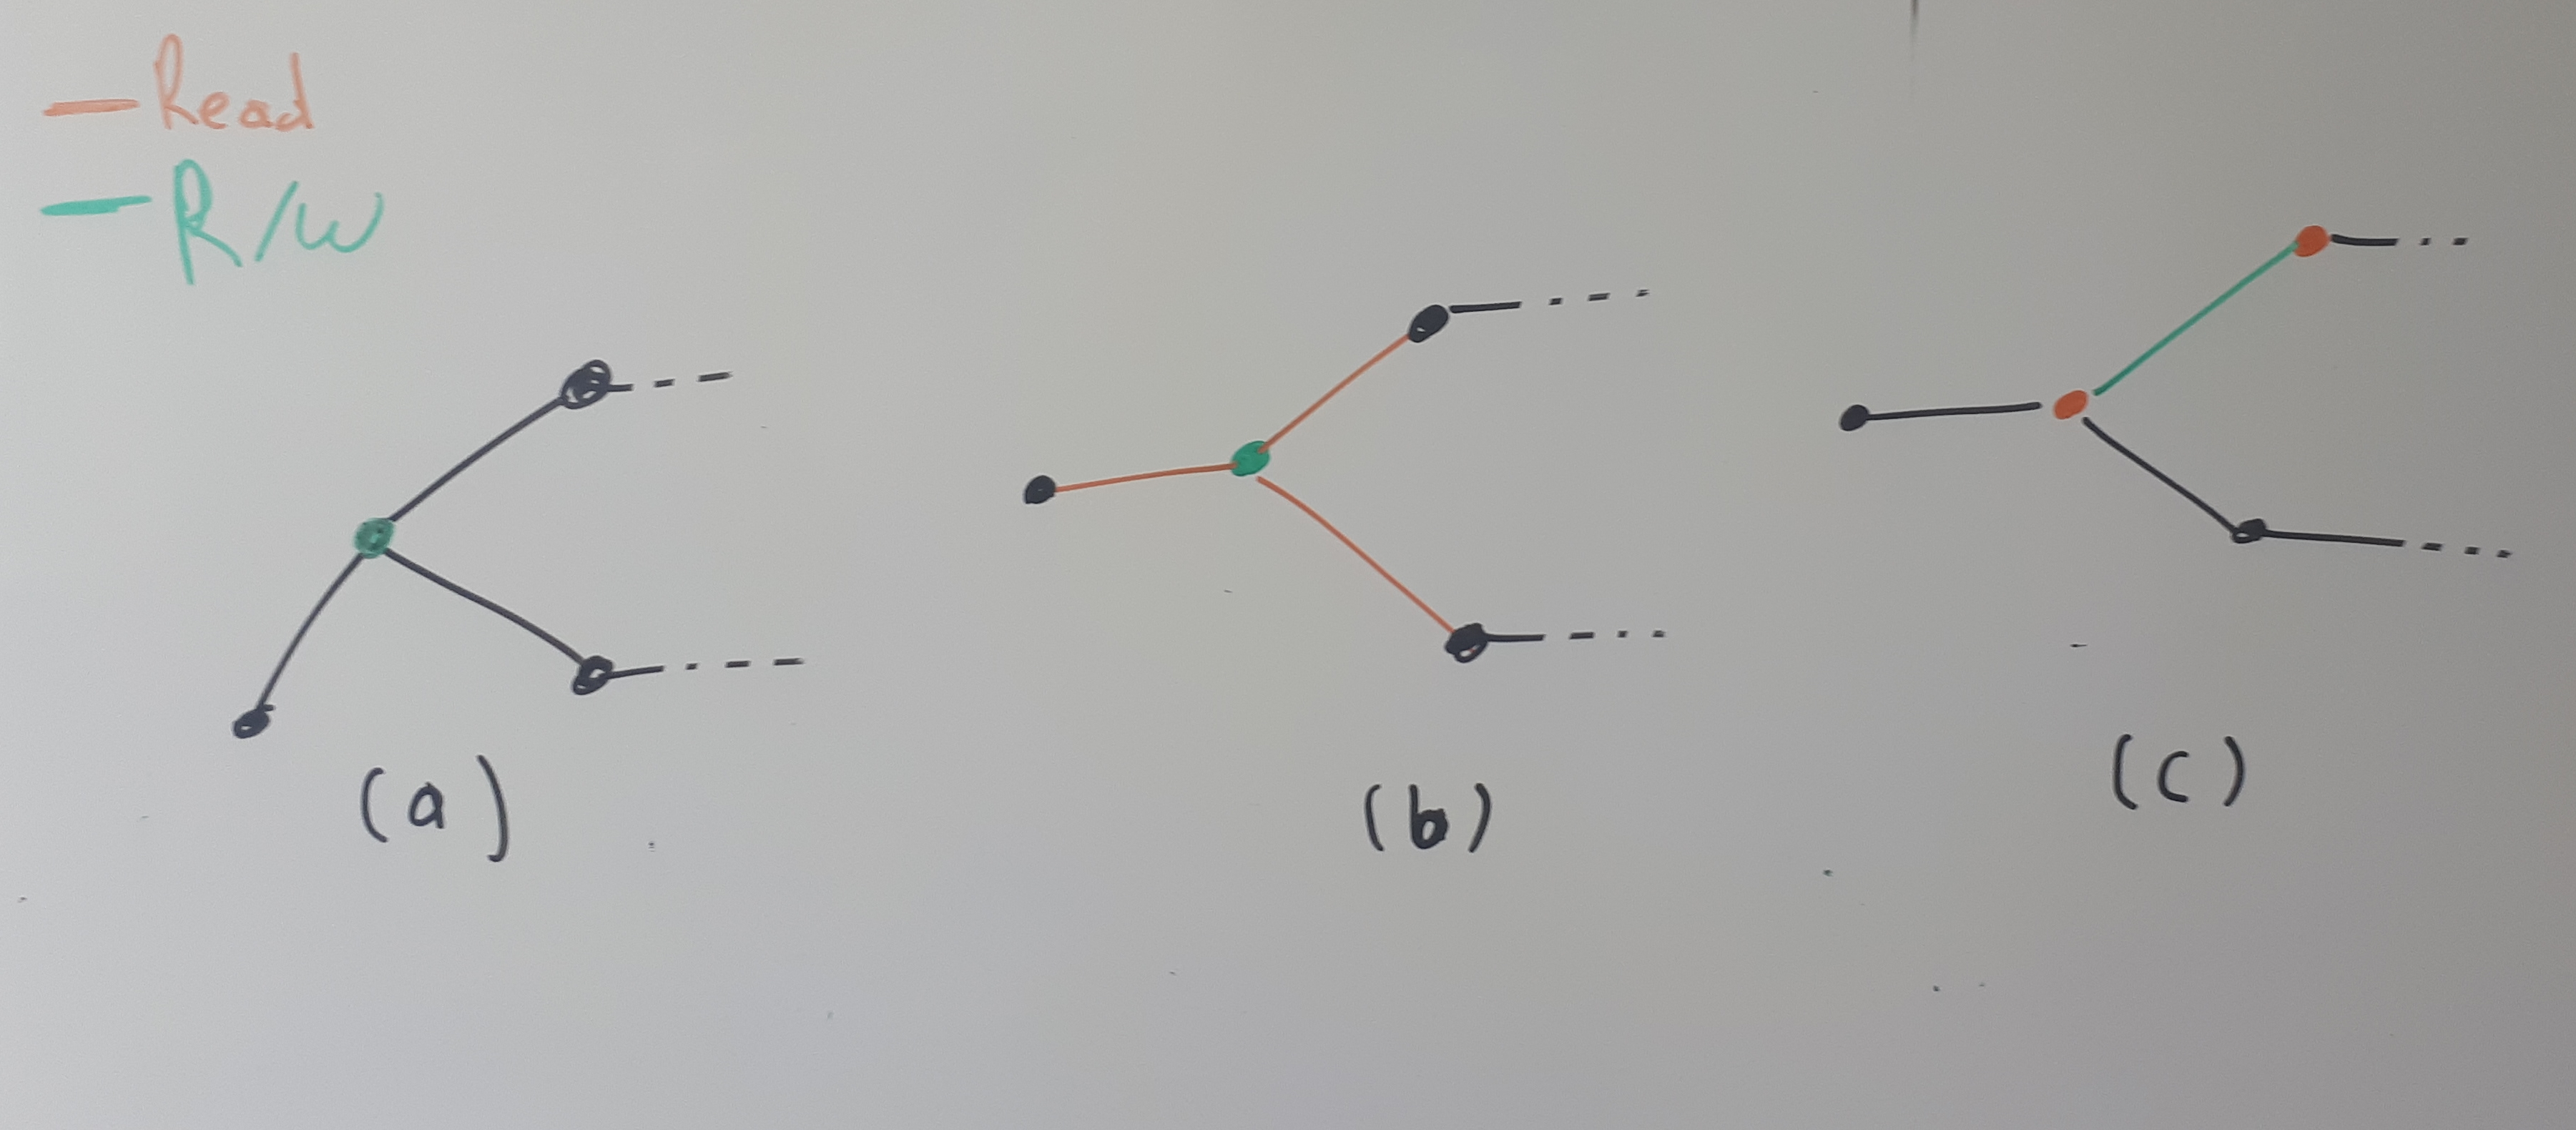
\includegraphics[width=\textwidth]{img/parcours_mesh}
	\caption{Accès aux données lors des parcours du réseau de dislocations}
	\label{fig:parcours_mesh}
\end{figure}

Les schémas d'accès aux données des différents parcours sont illustrés dans la figure \ref{fig:parcours_mesh}.


\subsubsection{Itération sur les nœuds}

Une fonction permet d'itérer sur les nœuds. Elle est équivalente à l'utilisation des itérateurs, mais son implémentation peut être différente et donc plus performante. Son prototype est le suivant : 

\begin{minted}{cpp}
	void fastIterate_nodes(Mesh& m, Function f);
\end{minted}

avec f une fonction de prototype

\begin{minted}{cpp}
	void f( Mesh::NodeInfo_ref& n);
\end{minted}

Pour chaque nœud du réseau, on applique la fonction f qui applique une transformation avec un accès aux données comme illustré en figure \ref{fig:parcours_mesh}a.

\subsubsection{Itération sur les nœuds avec segments connectés}

Une fonction permet le parcours des nœuds avec connaissance des segment connectés.  Son prototype est le suivant:

\begin{minted}{cpp}
    void fastIterate_nodes_withSegments(Mesh& m, Function f);
\end{minted}
Avec f une fonction de prototype.
\begin{minted}{cpp}
    void f( Mesh::NodeInfo_ref& n, 
            const std::vector<MeshHelper::Connexion>& connexions);
\end{minted}

\todo[inline]{Détailler MeshHelper::Connexion}

\verb|MeshHelper::Connexion| est une structure qui contient les informations sur un segment connecté au nœud n. f peut accéder aux données du noeud en lecture/ecriture, et aux segments en lecture seule, comme illustré sans la figure \ref{fig:parcours_mesh}b.

\subsubsection{Itération sur les segments avec nœuds connectés}

Une fonction permet le parcours des segments avec les nœuds connectés. Son prototype est le suivant:

\begin{minted}{cpp}
    void fastIterate_segments([const] Mesh& m, Function f);
\end{minted}
Avec f une fonction de prototype.
\begin{minted}{cpp}
    void f( [const] Mesh::SegmentInfo_ref& s_info, 
             const  Mesh::NodeInfo& n1_info, const Mesh::NodeInfo& n2_info);
\end{minted}

Pour chaque segment du réseau, on applique f qui a accès au segment courant en lecture/écriture et aux nœuds connectés en lecture seule, comme illustré dans la figure \ref{fig:parcours_mesh}c. Il existe aussi une version qui ne modifie pas le réseau, qui prend un \verb|const Mesh&|.

